\clearpage
\subsection{An architecture and dataset atlas}
\label{app:architecture-atlas}
These seven pages retain the remaining distinct architecture and dataset views
from the accepted experimental collection. We plot the two diagnostics relevant
to the scalar edges, $\widehat\Lambda$ and $\widehat H$, over every saved
step-size/batch-size cell. Run-level statistics use final-three-available-checkpoint
pools before averaging, with varying checkpoint horizons for vision models.
Gray cells marked N/A have no gain estimate; they are not stability observations.
An E marks a recorded loss-cutoff escape, including any available pre-escape probes.
Colors use a signed logarithmic transform about zero or one, with panel-specific
ranges; numerical labels and colorbar ticks remain in the original units.
A trailing $+$ or $-$ preserves the side of a reference after rounding.
The archive provenance retains the original source figure, checkpoint windows,
missing cells, and every displayed numerical value.

\begin{figure}[!ht]
\centering
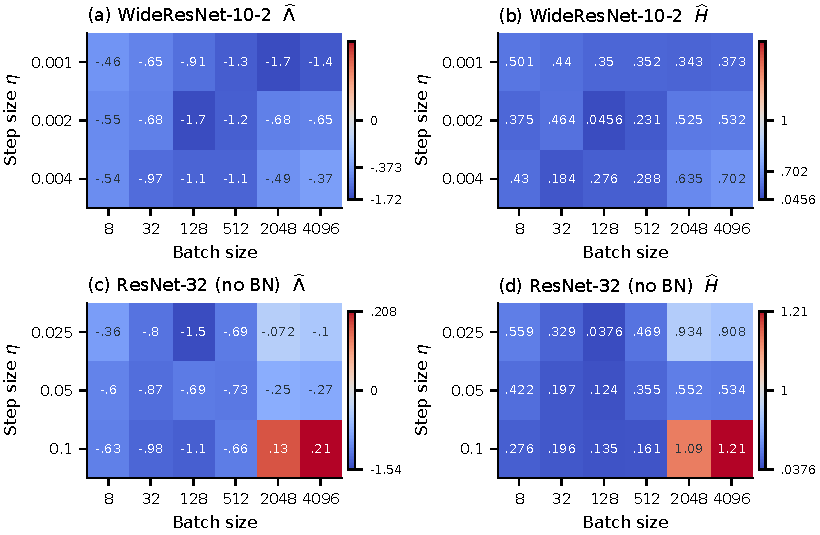
\includegraphics[width=\linewidth]{figures/empirical_atlas_01_residual_new.pdf}
\caption{\textbf{New residual-network sweeps on CIFAR-10.}
WideResNet-10-2 with native Fixup initialization and ResNet-32 without BatchNorm;
plain SGD with squared loss on the fixed 8,192-example subset.
WideResNet's measured cells have negative scalar log gain and harmonic gain below one.
ResNet-32 crosses both scalar references at its largest step size and large batches.
Thus the main CNN/MLP comparison does not imply that all trained architectures
exceed either reference. These are local scalar diagnostics, not network product exponents.}
\label{fig:atlas-residual-new}
\end{figure}

\clearpage
\begin{figure}[!ht]
\centering
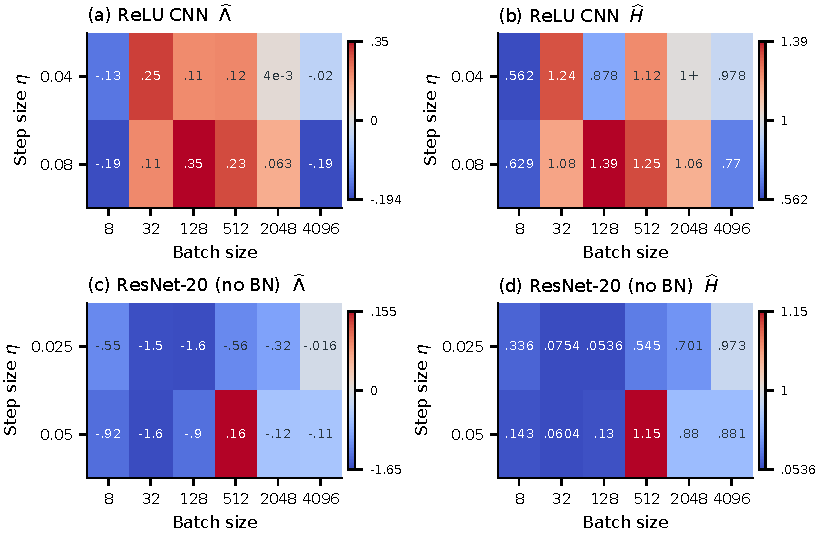
\includegraphics[width=\linewidth]{figures/empirical_atlas_02_archived_conv.pdf}
\caption{\textbf{Archived convolutional and residual architectures.}
ReLU CNN with three convolutional layers and ResNet-20 without BatchNorm,
using the same CIFAR-10 subset and squared-loss SGD objective.
The CNN contains positive-log-gain cells on either side of the harmonic reference;
for example $(\eta,B)=(0.04,128)$ has
$(\widehat\Lambda,\widehat H)\simeq(0.113,0.878)$.
ResNet-20 is mostly scalar-contracting in this grid, with a cell above both
references at $(0.05,512)$.
These archived measurements complement the new sweep and retain their original
checkpoint windows; they are not additional observations from the new continuations.}
\label{fig:atlas-archived-conv}
\end{figure}

\clearpage
\begin{figure}[!ht]
\centering
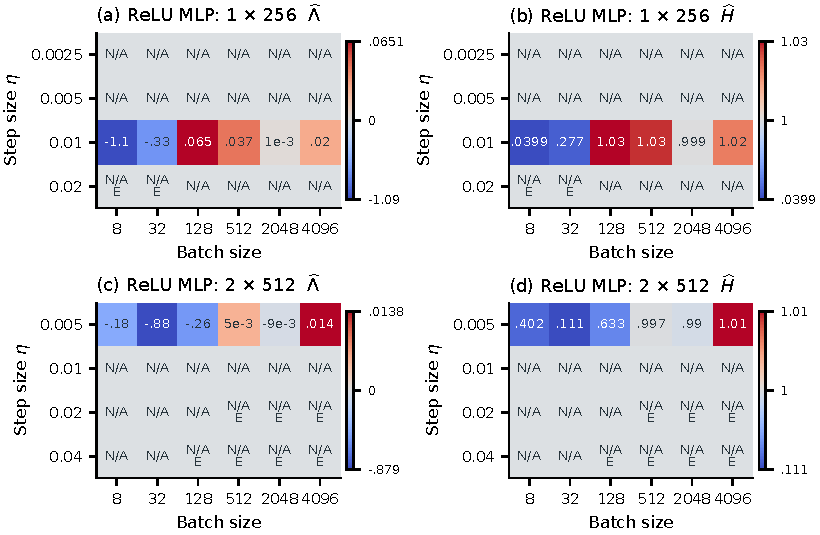
\includegraphics[width=\linewidth]{figures/empirical_atlas_03_shallow_mlp.pdf}
\caption{\textbf{Archived shallow ReLU MLPs, including incomplete diagnostic coverage.}
One hidden layer of width 256 and two hidden layers of width 512;
CIFAR-10 squared-loss SGD.
Only one learning-rate row per architecture has gain estimates in the accepted archive;
the other tested rows and recorded escapes remain visible as N/A and E.
For the measured one-layer row, the large-batch cells approach the scalar references:
at $(0.01,128)$, $(\widehat\Lambda,\widehat H)\simeq(0.0651,1.034)$.
The missing rows do not support interpolating a stability boundary or assigning
the architecture a universal regime.}
\label{fig:atlas-shallow-mlp}
\end{figure}

\clearpage
\begin{figure}[!ht]
\centering
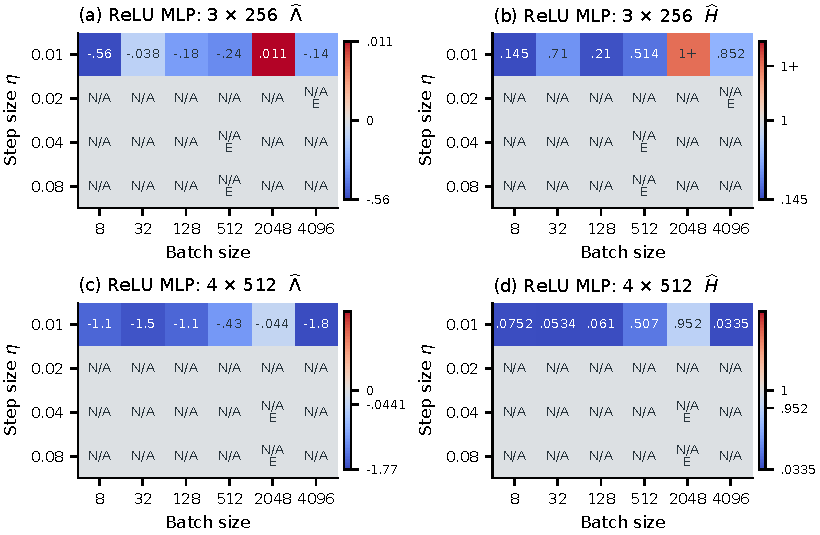
\includegraphics[width=\linewidth]{figures/empirical_atlas_04_deep_mlp.pdf}
\caption{\textbf{Archived deeper ReLU MLPs.}
Three hidden layers of width 256 and four hidden layers of width 512;
CIFAR-10 squared-loss SGD.
All available rows, missing gain estimates, and recorded escapes are retained.
The measured three-layer row includes both contracting cells and a large-batch cell
close to the two scalar references; the four-layer measured row is scalar-contracting.
The depth comparison also changes hidden width and should not be interpreted as
a controlled depth-only effect.}
\label{fig:atlas-deep-mlp}
\end{figure}

\clearpage
\begin{figure}[!ht]
\centering
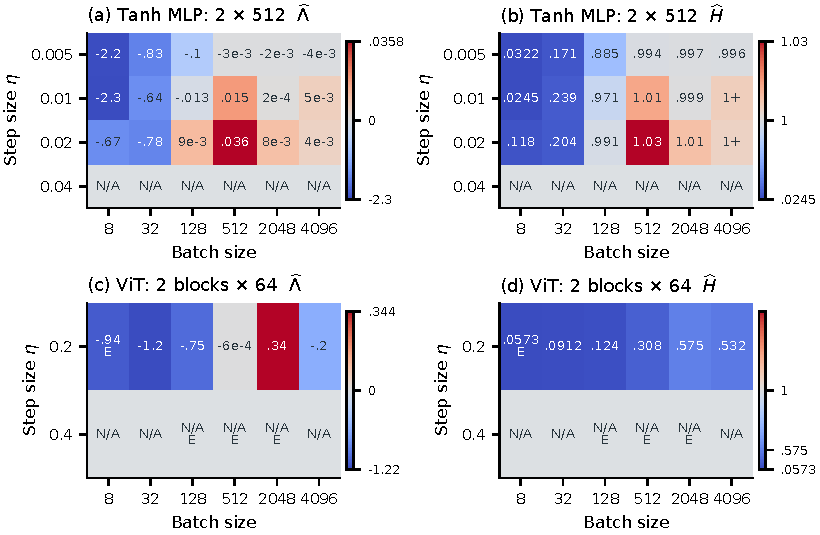
\includegraphics[width=\linewidth]{figures/empirical_atlas_05_tanh_vit.pdf}
\caption{\textbf{Archived tanh MLP and small vision transformer.}
Two hidden layers of width 512 with tanh activations, and a two-block width 64 ViT;
CIFAR-10 squared-loss SGD.
Several large-batch tanh settings approach the harmonic reference; at $(0.02,512)$,
$(\widehat\Lambda,\widehat H)\simeq(0.0358,1.0328)$.
The ViT at $(0.2,512)$ instead has log gain near zero while harmonic gain is substantially below one:
$(-0.000608,0.308)$.
Its $(0.2,2048)$ checkpoint pool is log-expanding with $\widehat H<1$.
These window-level differences illustrate distinct scalar regimes, while gray cells
and E annotations retain the archive's coverage and cutoff limitations.}
\label{fig:atlas-tanh-vit}
\end{figure}

\clearpage
\paragraph{Language-model metric definitions.}
The 168M-parameter decoder GPT is trained on a FineWeb-Edu subset using Adam
and mean token cross-entropy. Each run processes 16.384 million tokens with context 256;
the displayed pools combine checkpoints at 8.192, 12.288, and 16.384 million tokens.
Let $C_B$ be the Hessian or the positive-semidefinite generalized Gauss--Newton matrix (GGN).
Raw curvature uses $s_B=g_B^\top C_Bg_B/(g_B^\top g_B)$;
the raw gain $1-\eta s_B$ is an SGD counterfactual at an Adam-trained checkpoint.
It is not an Adam stability multiplier.

\begin{figure}[!ht]
\centering
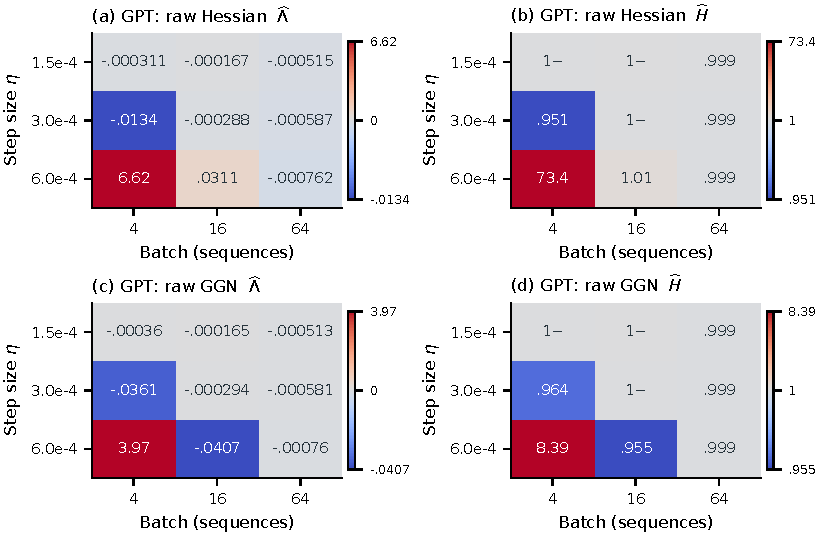
\includegraphics[width=\linewidth]{figures/empirical_atlas_06_gpt_raw.pdf}
\caption{\textbf{GPT/FineWeb-Edu: raw Hessian and GGN scalar views.}
The same nine parent hyperparameter cells underlie both views.
Batch size counts 256-token sequences, and equal processed-token budgets imply
different optimizer-update counts across batch sizes.
The largest-step, smallest-batch corner is strongly expanding in both views;
the exact Hessian and PSD GGN otherwise need not give the same scalar regime.
Per-run pools contain only 48 Hessian or 24 GGN draws, so inverse moments remain exploratory.
The extreme values are retained without clipping.
These counterfactual scalar grids neither measure a full-Adam Jacobian nor
establish a language model's asymptotic stability boundary.}
\label{fig:atlas-gpt-raw}
\end{figure}

\clearpage
\paragraph{Frozen Adam geometry.}
Freeze the bias-corrected Adam second-moment preconditioner
$D=\operatorname{diag}[(\sqrt{\widehat v}+\epsilon)^{-1}]$ at the checkpoint.
The frozen-metric scalar curvature is
\[
 s_{D,B}=\frac{(Dg_B)^\top C_B(Dg_B)}{g_B^\top Dg_B},
 \qquad a_{D,B}=1-\eta s_{D,B}.
\]
This is a symmetric-curvature Rayleigh quotient after a fixed change of coordinates.
It omits both momentum dynamics and derivatives of the evolving preconditioner.
The four GPT views are therefore distinct diagnostics of the same trained parents,
not four architectures or four independent empirical replications.

\begin{figure}[!ht]
\centering
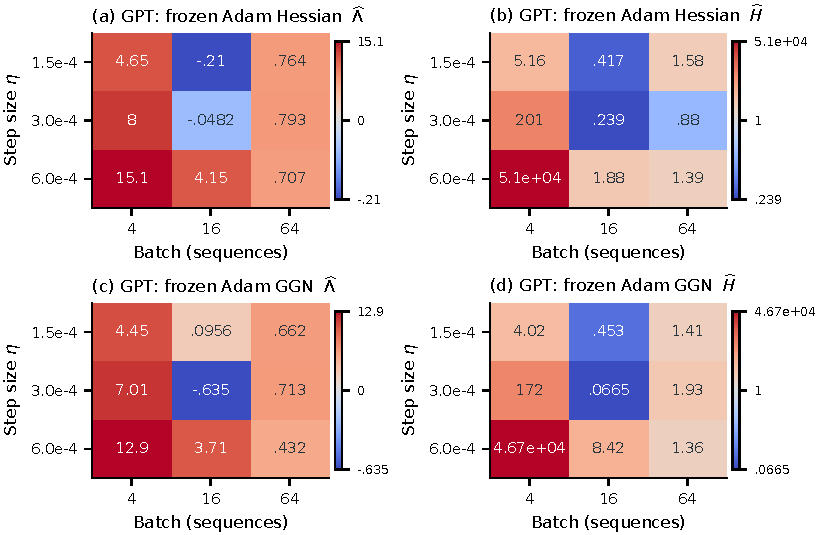
\includegraphics[width=\linewidth]{figures/empirical_atlas_07_gpt_frozen.pdf}
\caption{\textbf{GPT/FineWeb-Edu: frozen-Adam Hessian and GGN views.}
Changing the frozen geometry changes the scalar regime map.
For example, the frozen-GGN cell at $(\eta,B)=(0.0003,16)$ has
$\widehat\Lambda\simeq-0.635$ and $\widehat H\simeq0.0665$,
whereas other cells exceed both scalar references, some by large margins.
All values use the same token-aligned pools and optimizer limitations as
Figure~\ref{fig:atlas-gpt-raw}.
Local scalar expansion in these grids cannot be identified with instability
of the full Adam state, and no stationary bimodal language-model law is claimed.}
\label{fig:atlas-gpt-frozen}
\end{figure}
\clearpage
